\documentclass[../notes.tex]{subfiles}

\pagestyle{main}
\renewcommand{\chaptermark}[1]{\markboth{\chaptername\ \thechapter\ (#1)}{}}
\setcounter{chapter}{5}

\begin{document}




\chapter{Deviations from Ideality}
\section{Thermodynamics of the Rubber Band}
\begin{itemize}
    \item \marginnote{2/14:}Midterm:
    \begin{itemize}
        \item Take for two hours, any two hours tomorrow.
        \item Upload a single PDF file for your answer.
        \item Do not discuss the questions with anybody.
    \end{itemize}
    \item \textbf{Standard Gibbs free energy} (at $T$): The following energy, where $H^\circ(T)$ is the standard enthalpy at $T$ and $S^\circ(T)$ is the standard entropy at $T$. \emph{Denoted by} $\bm{G^\circ(T)}$. \emph{Given by}
    \begin{equation*}
        G^\circ(T) = H^\circ(T)-TS^\circ(T)
    \end{equation*}
    \begin{itemize}
        \item It follows that since the enthalpy is taken at constant pressure and the entropy $S(T,P)$ at nonstandard pressure is given by $S(T,P)=S^\circ(T)+R\ln P/P_0$ that the Gibbs free energy $S(T,P)$ at nonstandard pressure is
        \begin{align*}
            G(T,P) &= H^\circ(T)-TS(T,P)\\
            &= H^\circ(T)-T\left( S^\circ(T)+R\ln\frac{P}{P_0} \right)\\
            &= G^\circ(T)-RT\ln\frac{P}{P_0}
        \end{align*}
    \end{itemize}
    \item Gibbs free energy and equilibrium at constant $T,P$.
    \begin{itemize}
        \item If
        \begin{equation*}
            \ce{$a$A + $b$B -> $c$C + $d$D}
        \end{equation*}
        is in equilibrium where $A,B,C,D$ are ideal gases, then $\Delta G=0$.
        \item This implies that
        \begin{equation*}
            a\Delta G_a+b\Delta G_b = c\Delta G_c+d\Delta G_d
        \end{equation*}
        which is the \textbf{law of mass action}.
    \end{itemize}
    \item Example of phase equilibrium ($G(T)$ for solid/liquid/gas phases).
    \begin{itemize}
        \item We have from the total differential of $G$ that
        \begin{equation*}
            \left( \pdv{G}{T} \right)_P = -S
        \end{equation*}
        \item Since $S\geq 0$ always, $G$ is monotonically decreasing.
        \item During the liquid phase, there is a relatively constant slight negative slope in the $G(T)$ graph.
        \item During the gas phase, $S$ is much bigger, so there is a larger negative slope in the $G(T)$ graph.
        \item Additionally, at the heats of vaporization and fusion, the system is in equilibrium (hence the energies are the same), so the graph is continuous.
    \end{itemize}
    \item Rubber band temperature analysis.
    \begin{itemize}
        \item A rubber band heats up when stretched:
        \begin{itemize}
            \item We have that $\dd{U}=T\dd{S}+f\dd{L}$.
            \item We want to show that $(\pdv*{U}{L})_T=T(\pdv*{S}{L})_T+f$.
            \begin{align*}
                \dd{U} &= T\left( \pdv{S}{T} \right)_L\dd{T}+\left( \pdv{S}{L} \right)_T\dd{L}+f\dd{L}\\
                &= T\left( \pdv{S}{T} \right)_L\dd{T}+\left[ \left( \pdv{S}{L} \right)_T+f \right]\dd{S}
            \end{align*}
            \item All that's left is to show that $-(\pdv*{S}{L})_T=(\pdv*{f}{T})_L$, which we can do using Maxwell relations.
            \begin{equation*}
                \dd{A} = -S\dd{T}+f\dd{L}
            \end{equation*}
            \begin{equation*}
                \left( \pdv{U}{L} \right)_T = -T\left( \pdv{f}{T} \right)_L+f
            \end{equation*}
        \end{itemize}
        \item Stating the equation of state for the "ideal" rubber band.
        \begin{equation*}
            f = T\phi(L)
        \end{equation*}
        \begin{itemize}
            \item It follows that $(\pdv*{f}{T})_L=f/T$, and $(\pdv*{U}{L})_T=-T\cdot f/T+f=0$.
        \end{itemize}
        \item We are now ready to answer the question of does it cool down or heat up when stretched adiabatically.
        \begin{align*}
            \dd{U} = \left( \pdv{U}{L} \right)_T\dd{L}+\left( \pdv{U}{T} \right)_L\dd{T} &= \var{q}+f\dd{L}\\
            \left( \pdv{U}{T} \right)_L\dd{T} &= f\dd{L}\\
            C_L\dd{T} &= f\dd{L}\\
            \dd{T} &= \frac{f}{C_L}\dd{L} > 0
        \end{align*}
        so since $\dd{T}>0$, the rubber band heats up as it stretches.
        \item For intuitive motivation, PGS discusses Figure 17.1 of \textcite{bib:APChemNotes}.
    \end{itemize}
    \item Building a statistical model of the rubber band.
    \begin{itemize}
        \item Consider the rubber band to be made up of segments (you can think of each segment as part of a polymer). These segments can be oriented up or down. In a stretched rubber band, the polymers will be straight, i.e., all the segments will point the same way.
        \item The difference in energy $\Delta E$ between a segment (of length $\ell_0$) pointing up or down is $2f$.
        \item Thus, the partition function for each segment is
        \begin{equation*}
            q = \e[-f\ell_0/\kB T]+\e[f\ell_0/\kB T]
        \end{equation*}
        \begin{itemize}
            \item Note that this is the same as the partition function for a paramagnet (which can also either be up or down) except that $f\ell_0$ becomes $\mu_BB_z$.
        \end{itemize}
        \item When we sum the energies, we multiply the component partition functions. Thus,
        \begin{equation*}
            Q = q^N
        \end{equation*}
        \item We know that
        \begin{equation*}
            L = N(p+p_0+p-(-p_0))
            = Np_0(p+(-p))
            = N\ell_0\tanh\left( \frac{f\ell_0}{\kB T} \right)
        \end{equation*}
    \end{itemize}
\end{itemize}



\section{Van der Waals Phase Transitions}
\begin{itemize}
    \item \marginnote{2/16:}Wrapping up the rubber band analysis.
    \item Note that we can approximate $\tanh x\approx x$ for small $x$. Thus,
    \begin{equation*}
        L = N\ell_0\cdot\frac{f\ell_0}{\kB T}
    \end{equation*}
    for small $f$.
    \item Therefore, statistical mechanics predicts the rubber band "ideal" equation of state, $f=T\phi(L)$, where $f$ is the stretching force. Note that this is not at all like a mechanical spring constant; it is purely an entropy effect.
    \begin{itemize}
        \item $\dd{S}=\dd{S_\text{orientation}}+\dd{S_\text{thermal}}=\dd{S_\text{orientation}}+C/T\dd{T}$.
        \item $\dd{U}=C\dd{T}+T\dd{S}=0$, implying that $\dd{T}=-T/C\dd{S}$.
    \end{itemize}
    \item Adiabatic stretching decreases orientation entropy and increases the temperature.
    \item The same model predicts the Curie law of paramagnetism, $M=CB/T$.
    \begin{itemize}
        \item We have
        \begin{align*}
            M &= N\mu\tanh\frac{\mu B}{\kB T}\\
            M &= \frac{N\mu^2}{\kB}\frac{B}{T}
        \end{align*}
        where the second equation only holds for small $B$.
    \end{itemize}
    \item Adiabatic demagnetization allows you to go from \SI{4}{\kelvin} to \SI{1}{\kelvin} using \ce{He4} to \ce{He3} liquefaction. Adiabatic demagnetization increases spin entropy and reduces the temperature.
    \begin{itemize}
        \item To achieve \SI{4}{\kelvin}, we let \ce{He4} adiabatically expand, which makes it very cold. However, at temperatures below \SI{4}{\kelvin}, \ce{He4} is a liquid and it can no longer adiabatically expand like a gas.
        \item To achieve temperatures lower than \SI{4}{\kelvin}, you stick copper salt in a cryostat, subject it to a magnetic field, and cool it to \SI{4}{\kelvin} with the above method. The magnet aligns the spins. When you take the salt out of the magnetic field, the spins will randomize entropically, but this takes energy. You use the lattice energy to raise the spin energy.
    \end{itemize}
    \item The challenge of protein folding and structure determination.
    \begin{itemize}
        \item We have $\Delta G=\Delta(H-TS)$.
        \item Protein folding necessitates $\Delta S<0$ (you are creating order). Thus, we must have $\Delta H<\Delta(TS)=T\Delta S$, i.e., the protein must adopt a very, very stable conformation.
        \item Estimating $\Delta S$:
        \begin{equation*}
            \Delta S = \kB\ln W
            = \kB\ln 3^{100}
            = \SI{914}{\joule\per\kelvin\per\mole}
        \end{equation*}
        \begin{itemize}
            \item Using \textbf{Levinthal's paradox}, we can estimate the number of possible configurations of a protein.
            \item Each segment (essentially a \ce{C-C} bond) has about three dihedral angle possibilities for the segments at either end.
            \item Thus, for a protein that is 100 segments long, $W\approx 3^{100}$.
        \end{itemize}
        \item At \SI{300}{\kelvin}, $T\Delta S=\SI[per-mode=symbol]{274}{\kilo\joule\per\mole}$.
        \begin{itemize}
            \item It doesn't take much of a temperature difference to alter or prevent protein folding.
        \end{itemize}
        \item About 15 hydrogen bonds or a single disulfide bond is about \SI[per-mode=symbol]{274}{\kilo\joule\per\mole} of energy, so we can find ways to stabilize proteins over the entropic barriers.
        \item Just recently, a UChicago grad student (who had been working with a UChicago professor who's been studying the protein folding problem for a long time) headed a team at Google that has an AI that looks like it will be able to solve the protein folding problem.
    \end{itemize}
    \item \textbf{Levinthal's paradox}: The observation that finding the native folded state of a protein by a random search among all possible configurations can take an enormously long time. Yet proteins can fold in seconds or less.
    \item Real gases deviate from ideality due to molecular interactions.
    \item \textbf{Compressibility factor}: \emph{Denoted by} $\bm{z}$. \emph{Given by}
    \begin{equation*}
        z = \frac{P\overline{V}}{RT}
    \end{equation*}
    \item The van der Waals equation of state (where $\overline{V}$ is the molar volume):
    \begin{equation*}
        \left( P+\frac{a}{\overline{V}^2} \right)(\overline{V}-b) = RT
    \end{equation*}
    \begin{itemize}
        \item We can also rewrite this as
        \begin{equation*}
            P = \frac{RT}{\overline{V}-b}-\frac{a}{\overline{V}^2}
        \end{equation*}
        \item Note that $a,b\geq 0$.
        \item The compressibility is
        \begin{equation*}
            z = \frac{\overline{V}}{\overline{V}-b}-\frac{a}{RT\overline{V}}
        \end{equation*}
    \end{itemize}
    \item The van der Waals equation of state is cubic in $\overline{V}$ and can predict two different molar volumes (gas and liquid) for one pressure.
    \begin{figure}[h!]
        \centering
        \begin{tikzpicture}[
            xscale=10,yscale=0.03,
            every node/.style={black}
        ]
            \small
            \draw [stealth-stealth] (0,120) -- node[left]{$P$} (0,0) -- node[below]{$\overline{V}$} (0.6,0);
    
            \draw [blx,thick] plot[domain=0.0672:0.6,smooth,samples=500,/pgf/fpu,/pgf/fpu/output format=fixed] (\x,{(-0.0821*273*\x*\x+3.59*\x-3.59*0.0427)/(0.0427*\x*\x-\x*\x*\x)});
            \draw [blx,semithick] (0.0773,47.1) -- (0.3017,47.1);
    
            \footnotesize
            \node [below left] at (0.0672,119.849) {L};
            \node [below] at (0.092,30.481) {C};
            \node [left] at (0.0773,47.1) {D};
            \node [above] at (0.1959,52.755) {B};
            \node [above right] at (0.3017,47.1) {A};
            \node [below left] at (0.6,30.245) {G};
        \end{tikzpicture}
        \caption{The van der Waals isotherm of \ce{CO2} at \SI{0}{\celsius}.}
        \label{fig:vanDerWaalsIsotherm}
    \end{figure}
    \begin{itemize}
        \item We have that
        \begin{align*}
            RT &= \left( P+\frac{a}{\overline{V}^2} \right)(\overline{V}-b)\\
            &= P\overline{V}-bP+\frac{a}{\overline{V}}-\frac{ab}{\overline{V}^2}\\
            \frac{RT\overline{V}^2}{P} &= \overline{V}^3-b\overline{V}^2+\frac{a}{P}\overline{V}-\frac{ab}{P}\\
            0 &= \overline{V}^3-\left( b+\frac{RT}{P} \right)\overline{V}^2+\frac{a}{P}\overline{V}-\frac{ab}{P}
        \end{align*}
        \item Since it is cubic in $\overline{V}$, this means we can have up to three different molar volumes for one pressure.
        \item This also reflects the fact that as we compress a gas, it behaves ideally for a while, and then pressure is constant as condensation takes hold, and then we must apply massive amounts of pressure to make the volume any smaller.
        \item On $\overline{\text{AG}}$, the system is a gas. On $\overline{\text{LD}}$, it is a liquid. On $\overline{\text{AD}}$, pressure is constant as we compress more and more because condensation takes hold, so highly compressed gas molecules become liquid, reducing the pressure.
        \item Drawing the line $\overline{\text{AD}}$: The points at which gas stops and liquid starts must be at the same pressure.
        \item We must also have the area above and below the line equal (\textbf{Maxwell equal area construction}).
        \begin{itemize}
            \item Phase equilibrium (like we have along $\overline{\text{AD}}$) means that free energy does not change. Mathematically, $\Delta G(\text{A})=\Delta G(\text{D})$.
            \item If A and D represent gas and liquids at the same temperature, they are in equilibrium and they must have the same molar Gibbs free energy.
            \item We have $\dd{G}=-S\dd{T}+V\dd{P}$.
            \item Since $T$ is constant (this is an isotherm), $\dd{G}=V\dd{P}$.
            \item Thus, we can integrate along the curve $\overline{\text{DA}}$ to find an appropriate $\overline{\text{DA}}$ such that the integral is zero.
            \begin{align*}
                0 &= \Delta G(\text{A})-\Delta G(\text{D})\\
                &= \int_\text{D}^\text{A}\dd{G}\\
                &= \int_\text{D}^\text{A}V\dd{P}
            \end{align*}
            \item See Problem 23-46 for the "Maxwell equal area construction rule."
        \end{itemize}
    \end{itemize}
\end{itemize}



\section{More van der Waals Phenomena}
\begin{itemize}
    \item \marginnote{2/18:}The cubic vdW equation of state predicts a critical point at $T_c$ at and above which only one $P$ for $(V,T)$ solution is possible.
    \begin{itemize}
        \item The behavior of isotherms around the critical temperature.
        \begin{itemize}
            \item For isotherms below the critical temperature, there will be a range of volumes where the gas and liquid phases are in equilibrium.
            \item For isotherms above the critical temperature, we only have the gas phase, so there is no region of constant pressure as we compress the system.
            \item This means that at the critical temperature $T=T_c$, there will only be a single volume $V_c$ and hence pressure $P_c$ at which the gas and liquid phases are in equilibrium. Mathematically, this means that each of the three roots of the cubic van der Waals equation exist at the same point $V_c$, i.e., that the equation is of the form $(V-\overline{V}_c)^3$.
        \end{itemize}
        \item Expanding, we have
        \begin{align*}
            0 &= \overline{V}^3-\left( b+\frac{RT}{P} \right)\overline{V}^2+\frac{a}{P}\overline{V}-\frac{ab}{P}\\
            &= \overline{V}^3-3\overline{V}_c\overline{V}^2+3\overline{V}_c^2\overline{V}-\overline{V}_c^3
        \end{align*}
        \item Thus, at $T_c$,
        \begin{align*}
            b+\frac{RT_c}{P_c} &= 3\overline{V}_c&
            \frac{a}{P_c} &= 3V_c^2&
            \frac{ab}{P_c} &= \overline{V}_c^3
        \end{align*}
        \item One immediate consequence is that
        \begin{align*}
            \overline{V}_c^3 &= \frac{a}{P_c}\cdot b\\
            \overline{V}_c^3 &= 3V_c^2b\\
            \overline{V}_c &= 3b
        \end{align*}
        \begin{itemize}
            \item Thus, the critical volume is on the order of magnitude of the molecular volume.
            \item Note that we can't manipulate the first equation into a different relation between $\overline{V}_c$ and $b$ using the ideal gas law substitution because this is a van der Waals gas.
        \end{itemize}
        \item It follows that
        \begin{align*}
            3V_c^2 &= \frac{a}{P_c}&
                b+\frac{RT_c}{P_c} &= 3\overline{V}_c\\
            P_c &= \frac{a}{3(3b)^2}&
                b+RT_c\cdot\frac{27b^2}{a} &= 3(3b)\\
            P_c &= \frac{a}{27b^2}&
                T_c &= \frac{8a}{27Rb}
        \end{align*}
        \item Thus,
        \begin{equation*}
            z_c = \frac{P_cV_c}{RT_c} = \frac{3}{8}
        \end{equation*}
        \begin{itemize}
            \item Indeed, the vdW equation predicts the compressibility at the critical point to be $3/8$. The Redlich-Kwong predicts $1/3$. The Peng-Robinson predicts $0.307$. The experimental values are around $0.3$. Water and ammonia deviate significantly: $0.23$ and $0.24$, respectively, due to their strong dipole moments/hydrogen bonding. Table 16.5 gives a lot of related data.
        \end{itemize}
        \item Also, at $T_c,V_c$, we have that $(\pdv*{P}{V})_T=0$ and $\kappa\to\infty$ (recall that $\kappa$ is the isothermal compressibility).
        \begin{itemize}
            \item It follows from the vdW that $\kappa\propto(\overline{V}-\overline{V}_c)^{-1}$.
            \item Experimental value: \emph{Every} gas satisfies $\kappa\propto(\overline{V}-\overline{V}_c)^{-1.24}$.
            \item The mystery was solved theoretically in the 1970s with renormalization group theory.
        \end{itemize}
    \end{itemize}
    \item Law of corresponding states.
    \begin{itemize}
        \item We define the reduced pressure, volume, and temperature by
        \begin{align*}
            P_R &= \frac{P}{P_c}&
            V_R &= \frac{V}{V_c}&
            T_R &= \frac{T}{T_c}
        \end{align*}
        \item Note that
        \begin{equation*}
            \frac{RT}{P_cV_c} = \frac{RT_c}{P_cV_c}\frac{T}{T_c}
            = \frac{1}{z_c}\frac{T}{T_c}
            = \frac{8}{3}T_R
        \end{equation*}
        \item Thus,
        \begin{align*}
            RT &= \left( P+\frac{a}{\overline{V}^2} \right)(\overline{V}-b)\\
            &= \left( P+\frac{3\overline{V}_c^2P_c}{\overline{V}^2} \right)\left( \overline{V}-\frac{\overline{V}_c}{3} \right)\\
            \frac{RT}{P_cV_c} &= \left( \frac{P}{P_c}+\frac{3\overline{V}_c^2}{\overline{V}^2} \right)\left( \frac{\overline{V}}{\overline{V}_c}-\frac{1}{3} \right)\\
            \frac{8}{3}T_R &= \left( P_R+\frac{3}{\overline{V}_R^2} \right)\left( \overline{V}_R-\frac{1}{3} \right)
        \end{align*}
    \end{itemize}
    \item Virial expansion to experimentally determine the vdW coefficients $a,b$ from the compressibility near ideal conditions.
    \begin{itemize}
        \item We let
        \begin{equation*}
            z = 1+\frac{B_{2V}(T)}{\overline{V}}+\frac{B_{3V}(T)}{\overline{V}^2}+\cdots
        \end{equation*}
        where $B_{iV}(T)$ is the \textbf{$\bm{i^\textbf{th}}$ virial coefficient}.
        \item It follows that
        \begin{align*}
            \frac{P\overline{V}}{RT} &= \frac{\overline{V}}{\overline{V}-b}-\frac{a}{RT\overline{V}}\\
            &= \frac{1}{1-b/\overline{V}}-\frac{a}{RT\overline{V}}\\
            &= 1+\left( \frac{b}{\overline{V}}-\frac{a}{RT\overline{V}} \right)+\text{terms in }\tfrac{1}{\overline{V}^2}+\cdots
        \end{align*}
        where we get from the second to the third line using the expansion
        \begin{equation*}
            \frac{1}{1-x} = 1+x+x^2+\cdots
        \end{equation*}
        \item Thus,
        \begin{equation*}
            B_{2V}(T) = b-\frac{a}{RT}
        \end{equation*}
    \end{itemize}
    \item Microscopic origin of the vdW coefficients from the interaction potential.
    \begin{itemize}
        \item Draws the interaction potential for a diatomic molecule.
        \begin{itemize}
            \item The repulsion comes from the Fermi exclusion principle.
        \end{itemize}
        \item Discusses dipole-induced dipole moments.
        \begin{itemize}
            \item $-1/2\propto E^2\propto 1/r^6$.
        \end{itemize}
        \item The origin of vdW (or London dispersion) interaction is quantum mechanical.
        \begin{itemize}
            \item We use perturbation theory to calculate the interaction between two neighboring quantum dipoles.
            \begin{equation*}
                \Delta E^{(1)} = \ev{H_{int}}{\psi_A^\circ\psi_B^\circ} = 0
            \end{equation*}
            \item Thus we need the second order correction:
            \begin{equation*}
                \Delta E^{(2)} = -\sum_{ij}\frac{|\ev{H_{int}}{\psi_A^\circ\psi_B^\circ}|}{E_a^A+E_j^B-(E_0^A+E_0^B)} \approx -\frac{c}{r^6}
            \end{equation*}
            where $c\geq 0$.
        \end{itemize}
    \end{itemize}
\end{itemize}



\section{Office Hours (PGS)}
\begin{itemize}
    \item Integrating along the curve in Figure \ref{fig:vanDerWaalsIsotherm}?
    \begin{itemize}
        \item Integrating along the curve with respect to $P$ means (geometrically) that we take the area "under" (to the left of) the curve from $A$ to $C$, then subtract the area under from $C$ to $B$, and then add the area under from $B$ to $A$. This calculation gets us overall the area of the bottom chunk as negative and the area of the top chunk as positive.
    \end{itemize}
\end{itemize}



\section{Chapter 16: The Properties of Gases}
\emph{From \textcite{bib:McQuarrieSimon}.}
\begin{itemize}
    \item \marginnote{2/21:}Outline:
    \begin{itemize}
        \item Having studied ad nauseam the properties of individual atoms and molecules, we now turn our attention to systems consisting of large numbers of atoms and molecules.
        \item The ideal gas equation is discussed, the van der Waals equation as the most famous extension of it, and then \textbf{virial expansions} as an even more systematic and accurate approach.
        \item Relating virial coefficients to the intermolecular interaction energy reveals that deviations from ideal gas behavior provide great insight into molecular interactions.
    \end{itemize}
    \item \textbf{Virial expansion}: An expression for the pressure of a gas as a polynomial in the density.
    \item \textbf{Ideal-gas equation of state}: An equation of state relating the pressure, volume, and temperature of a gas that is sufficiently dilute (i.e., with particles sufficiently far apart) for the intermolecular interactions to be negligible. \emph{Given by}
    \begin{align*}
        PV &= nRT&
        P\overline{V} &= RT
    \end{align*}
    \item \textbf{Ideal gas}: A gas that obeys the ideal-gas equation of state.
    \begin{itemize}
        \item All gases, regardless of the shape or size of the molecules or how the molecules interact with each other, behave ideally if they are sufficiently dilute.
        \item "Experimentally, most gases satisfy [the ideal-gas equation of state] to approximately $1\%$ at one atm and \SI{0}{\celsius}" \parencite[638]{bib:McQuarrieSimon}.
    \end{itemize}
    \item \textbf{Extensive quantity}: A quantity that is directly proportional to the size of the system in question. \emph{Also known as} \textbf{extensive variable}.
    \item \textbf{Intensive quantity}: A quantity that does not depend on the size of the system in question. \emph{Also known as} \textbf{intensive variable}.
    \item "If we divide an extensive quantity by the number of particles or the number of moles in a system, we obtain an intensive quantity" \parencite[638]{bib:McQuarrieSimon}.
    \item \textbf{Liter}: A unit of volume. \emph{Denoted by} \textbf{L}. \emph{Given by}
    \begin{equation*}
        \SI{1}{\liter} = \SI{1}{\deci\meter\cubed}
    \end{equation*}
    \begin{itemize}
        \item The SI unit of volume is \si{\cubic\meter}, but liters are an acceptable unit of volume in the IUPAC system.
    \end{itemize}
    \item \textbf{Pascal}: The SI unit of pressure. \emph{Denoted by} \textbf{Pa}. \emph{Given by}
    \begin{equation*}
        \SI{1}{\pascal} = \SI[per-mode=fraction,fraction-function=\tfrac]{1}{\newton\per\meter\squared}
        = \SI[per-mode=fraction,fraction-function=\tfrac]{1}{\kilo\gram\per\meter\per\second\squared}
    \end{equation*}
    \item "Pressure can be measured experimentally by observing how high a column of liquid (usually mercury) is supported by the gas" \parencite[638]{bib:McQuarrieSimon}.
    \begin{itemize}
        \item If $m$ is the mass of the liquid, $g$ is the \textbf{gravitational acceleration constant}, $A$ is the base area of the column, $\rho$ is the density of the liquid, and $h$ is the height of the column, then
        \begin{equation*}
            P = \frac{F}{A} = \frac{mg}{A} = \frac{\rho hAg}{A} = \rho hg
        \end{equation*}
    \end{itemize}
    \item \textbf{Gravitational acceleration constant}: The acceleration of an object due to gravity at the surface of the Earth. \emph{Denoted by} $\bm{g}$. \emph{Given by}
    \begin{equation*}
        g = \SI[per-mode=fraction,fraction-function=\tfrac]{9.8067}{\meter\per\second\squared}
    \end{equation*}
    \item The pressure exerted by a \SI{76.000}{\centi\meter} column of mercury ($\rho(\ce{Hg})=\SI{13.596}{\gram\per\cubic\centi\meter}$) is
    \begin{align*}
        P &= \rho gh\\
        &= \SI[per-mode=fraction,fraction-function=\tfrac]{1.0133e6}{\gram\per\centi\meter\per\square\second}\\
        &= \SI[per-mode=fraction,fraction-function=\tfrac]{1.0133e5}{\kilo\gram\per\meter\per\square\second}\\
        &= \SI{1.0133e5}{\pascal}\\
        &= \SI{101.33}{\kilo\pascal}
    \end{align*}
    \item \textbf{Atmosphere}: The pressure that supports a \SI{76.0}{\centi\meter} column of mercury. \emph{Denoted by} \textbf{atm}. \emph{Given by}
    \begin{equation*}
        \SI{1}{\atmosphere} = \SI{101.325}{\kilo\pascal}
    \end{equation*}
    \item \textbf{Bar}: The SI standard of pressure. \emph{Denoted by} \textbf{bar}. \emph{Given by}
    \begin{equation*}
        \SI{1}{\bar} = \SI{e5}{\pascal}
    \end{equation*}
    \item \textbf{Torr}: The pressure that supports a \SI{1.00}{\milli\meter} column of mercury. \emph{Denoted by} \textbf{torr}. \emph{Given by}
    \begin{equation*}
        \SI{1}{\torr} = \frac{1}{760}\,\text{atm}
    \end{equation*}
    \item "Because we are experiencing a transition period between the widespread use of \si{\atmosphere} and \si{\torr} on the one hand and the future use of \si{\bar} and \si{\kilo\pascal} on the other hand, students of physical chemistry must be proficient in both sets of pressure units" \parencite[639]{bib:McQuarrieSimon}.
    \item Temperatures as low as \SI{1e-7}{\kelvin} and as high as \SI{1e8}{\kelvin} have been achieved in the laboratory.
    \item \textbf{Triple point}: The point $(P,V,T)$ at which all three of a given substance's phases are in equilibrium.
    \item \textbf{Kelvin}: The SI unit of temperature, defined as $1/273.16$ of the temperature of the triple point of water. \emph{Denoted by} \textbf{K}.
    \item "We will use the lower case $t$ for \si{\celsius} and the upper case $T$ for \si{\kelvin}" \parencite[640]{bib:McQuarrieSimon}.
    \item \textbf{Room temperature}: The temperature $\SI{25}{\celsius}=\SI{298.15}{\kelvin}$.
    \item If we plot $P\overline{V}$ vs. $P$ for several gases at $T=\SI{273.15}{\kelvin}$, all the data can be extrapolated to a common value of $P\overline{V}=\SI{22.414}{\liter\atmosphere}$ as $P\to 0$. Thus,
    \begin{align*}
        R = \frac{P\overline{V}}{T} = \frac{\SI{22.414}{\liter\atmosphere}}{\SI{273.15}{\kelvin}} &= \SI[per-mode=fraction,fraction-function=\tfrac]{0.082058}{\liter\atmosphere\per\mole\per\kelvin}\\
        &= \SI[per-mode=fraction,fraction-function=\tfrac]{8.3145}{\joule\per\mole\per\kelvin}\\
        &= \SI[per-mode=fraction,fraction-function=\tfrac]{0.083145}{\liter\bar\per\mole\per\kelvin}
    \end{align*}
    \item \textbf{Compressibility factor}: The following quantity. \emph{Denoted by} $\bm{Z}$. \emph{Given by}
    \begin{equation*}
        Z = \frac{P\overline{V}}{RT}
    \end{equation*}
    \begin{figure}[h!]
        \centering
        \begin{subfigure}[b]{0.49\linewidth}
            \centering
            \begin{tikzpicture}[
                xscale=0.3,yscale=1.5,
                every node/.style=black
            ]
                \footnotesize
                \draw [stealth-stealth] (0,2.75) -- node[left=7mm]{$Z$} (0,0) -- node[below=6mm]{$P$ (bar)} (21,0);
                \foreach \x [evaluate=\x as \n using int(50*\x)] in {4,8,...,20} {
                    \draw (\x,0.05) -- ++(0,-0.1) node[below]{$\n$};
                }
                \foreach \y in {0.5,1.0,1.5,2.0,2.5} {
                    \draw (0.25,\y) -- ++(-0.5,0) node[left]{$\y$};
                }
                \node[below left=1mm]{0};
        
                \draw [thick] plot[smooth] coordinates {
                    (0 ,1.000)
                    (20,1.000)
                } node[right]{Ideal gas};
                \draw [blz,thick] plot[smooth] coordinates {
                    (0 ,1.000)
                    (1 ,1.037)
                    (2 ,1.083)
                    (3 ,1.134)
                    (4 ,1.184)
                    (5 ,1.228)
                    (6 ,1.267)
                    (7 ,1.302)
                    (8 ,1.332)
                    (9 ,1.359)
                    (10,1.384)
                    (11,1.406)
                    (12,1.427)
                    (13,1.446)
                    (14,1.467)
                    (15,1.480)
                    (16,1.496)
                    (17,1.511)
                    (18,1.525)
                    (19,1.538)
                    (20,1.551)
                } node[right]{\ce{He}};
                \draw [bly,thick] plot[smooth] coordinates {
                    (0 ,1.000)
                    (1 ,0.917)
                    (2 ,0.856)
                    (3 ,0.832)
                    (4 ,0.844)
                    (5 ,0.881)
                    (6 ,0.932)
                    (7 ,0.991)
                    (8 ,1.053)
                    (9 ,1.118)
                    (10,1.184)
                    (11,1.250)
                    (12,1.317)
                    (13,1.384)
                    (14,1.451)
                    (15,1.518)
                    (16,1.585)
                    (17,1.652)
                    (18,1.718)
                    (19,1.784)
                    (20,1.850)
                } node[right,yshift=-1.3mm]{\ce{CH4}};
                \draw [blx,thick] plot[smooth] coordinates {
                    (0 ,1.000)
                    (1 ,0.988)
                    (2 ,0.993)
                    (3 ,1.022)
                    (4 ,1.068)
                    (5 ,1.123)
                    (6 ,1.181)
                    (7 ,1.240)
                    (8 ,1.297)
                    (9 ,1.353)
                    (10,1.408)
                    (11,1.461)
                    (12,1.512)
                    (13,1.563)
                    (14,1.612)
                    (15,1.660)
                    (16,1.706)
                    (17,1.752)
                    (18,1.797)
                    (19,1.840)
                    (20,1.883)
                } node[right,yshift=1.3mm]{\ce{N2}};
            \end{tikzpicture}
            \caption{Changing the gas type.}
            \label{fig:ZvsPa}
        \end{subfigure}
        \begin{subfigure}[b]{0.49\linewidth}
            \centering
            \begin{tikzpicture}[
                xscale=0.3,yscale=1.5,
                every node/.style=black
            ]
                \footnotesize
                \draw [stealth-stealth] (0,2.75) -- node[left=7mm]{${\color{white}Z}$} (0,0) -- node[below=6mm]{$P$ (bar)} (21,0);
                \foreach \x [evaluate=\x as \n using int(50*\x)] in {4,8,...,20} {
                    \draw (\x,0.05) -- ++(0,-0.1) node[below]{$\n$};
                }
                \foreach \y in {0.5,1.0,1.5,2.0,2.5} {
                    \draw (0.25,\y) -- ++(-0.5,0);
                }
                \node[below left=1mm]{0};
        
                \draw [blt,thick] plot[smooth] coordinates {
                    (0 ,1.000)
                    (1 ,1.005)
                    (2 ,1.014)
                    (3 ,1.025)
                    (4 ,1.039)
                    (5 ,1.056)
                    (6 ,1.074)
                    (7 ,1.095)
                    (8 ,1.117)
                    (9 ,1.140)
                    (10,1.165)
                    (11,1.191)
                    (12,1.217)
                    (13,1.244)
                    (14,1.272)
                    (15,1.300)
                    (16,1.329)
                    (17,1.358)
                    (18,1.387)
                    (19,1.417)
                    (20,1.447)
                } node[right]{\SI{600}{\kelvin}};
                \draw [blz,thick] plot[smooth] coordinates {
                    (0 ,1.000)
                    (1 ,0.977)
                    (2 ,0.965)
                    (3 ,0.964)
                    (4 ,0.974)
                    (5 ,0.993)
                    (6 ,1.020)
                    (7 ,1.053)
                    (8 ,1.089)
                    (9 ,1.129)
                    (10,1.172)
                    (11,1.215)
                    (12,1.260)
                    (13,1.306)
                    (14,1.353)
                    (15,1.400)
                    (16,1.447)
                    (17,1.495)
                    (18,1.542)
                    (19,1.591)
                    (20,1.638)
                } node[right]{\SI{400}{\kelvin}};
                \draw [bly,thick] plot[smooth] coordinates {
                    (0 ,1.000)
                    (1 ,0.917)
                    (2 ,0.856)
                    (3 ,0.832)
                    (4 ,0.844)
                    (5 ,0.881)
                    (6 ,0.932)
                    (7 ,0.991)
                    (8 ,1.053)
                    (9 ,1.118)
                    (10,1.184)
                    (11,1.250)
                    (12,1.317)
                    (13,1.384)
                    (14,1.451)
                    (15,1.518)
                    (16,1.585)
                    (17,1.652)
                    (18,1.718)
                    (19,1.784)
                    (20,1.850)
                } node[right]{\SI{300}{\kelvin}};
                \draw [blx,thick] plot[smooth] coordinates {
                    (0 ,1.000)
                    (0.25,0.915)
                    (0.50,0.820)
                    (0.75,0.706)
                    (0.80,0.680)
                    (0.85,0.652)
                    (0.90,0.622)
                    (0.95,0.589)
                    (1 ,0.553)
                    (1.05,0.513)
                    (1.10,0.468)
                    (1.15,0.423)
                    (1.20,0.386)
                    (1.25,0.365)
                    (1.30,0.355)
                    (1.35,0.350)
                    (1.40,0.348)
                    (1.45,0.349)
                    (1.50,0.351)
                    (1.55,0.353)
                    (1.60,0.357)
                    (1.65,0.361)
                    (1.70,0.365)
                    (1.75,0.370)
                    (2 ,0.397)
                    (3 ,0.517)
                    (4 ,0.637)
                    (5 ,0.755)
                    (6 ,0.870)
                    (7 ,0.983)
                    (8 ,1.094)
                    (9 ,1.203)
                    (10,1.310)
                    (11,1.416)
                    (12,1.521)
                    (13,1.626)
                    (14,1.729)
                    (15,1.831)
                    (16,1.933)
                    (17,2.034)
                    (18,2.135)
                    (19,2.235)
                    (20,2.334)
                } node[right]{\SI{200}{\kelvin}};
            \end{tikzpicture}
            \caption{Changing the gas temperature.}
            \label{fig:ZvsPb}
        \end{subfigure}
        \caption{Plots of the compressibility factor vs. pressure.}
        \label{fig:ZvsP}
    \end{figure}
    \begin{itemize}
        \item We use the compressibility factor, which is constant at 1 for an ideal gas, to visualize deviations from ideality for different gases (Figure \ref{fig:ZvsPa}) at different temperatures (Figure \ref{fig:ZvsPb}).
        \item At lower temperatures, intermolecular attraction takes hold, reducing the true volume and making $Z<1$.
        \item At higher temperatures, molecules are moving fast enough to make negligible their attractions. Here, only repulsions due to their nonzero volume take hold at higher pressures.
    \end{itemize}
    \item "The closer the gas is to the point at which it begins to liquify, the larger the deviations from ideal behavior will be" \parencite[642]{bib:McQuarrieSimon}.
    \item \textbf{Van der Waals equation}: The most well known of the gaseous equations of state which account for intermolecular interactions. \emph{Given by}
    \begin{equation*}
        \left( P+\frac{a}{\overline{V}^2} \right)(\overline{V}-b) = RT
    \end{equation*}
    \begin{itemize}
        \item Note that as $\overline{V}\to\infty$, the van der Waals equation becomes the ideal-gas equation of state.
        \item The van der Waals equation is also commonly written in the following form.
        \begin{equation*}
            P = \frac{RT}{\overline{V}-b}-\frac{a}{\overline{V}^2}
        \end{equation*}
    \end{itemize}
    \item \textbf{Van der Waals constants}: The constants $a,b$ in the van der Waals equation, the values of which depend upon the particular gas.
    \begin{itemize}
        \item We will see later that "the value of $a$ reflects how strongly the molecules of a gas attract each other and the value of $b$ reflects the size of the molecules" \parencite[643]{bib:McQuarrieSimon}.
        \item Table 16.3 lists van der Waals constants for various substances.
    \end{itemize}
    \item The van der Waals equation approximates the behavior depicted in Figure \ref{fig:ZvsP} since
    \begin{equation*}
        Z = \frac{P\overline{V}}{RT}
        = \frac{\overline{V}}{\overline{V}-b}-\frac{a}{RT\overline{V}}
    \end{equation*}
    \begin{itemize}
        \item At high pressures ($\overline{V}\to 0$), the first term above dominates because $\overline{V}-b$ gets really small.
        \item At low pressures, the second term dominates.
        \item Notice that this also relates to the previously mentioned roles of $a,b$ (e.g., at high pressures, the size of the molecules [and $b$] becomes significant).
    \end{itemize}
    \item To solve the van der Waals equation for a molar volume given the other state variables, we must find the roots of a cubic equation via Newtons' method.
    \begin{equation*}
        \overline{V}^3-\left( b+\frac{RT}{P} \right)\overline{V}^2+\frac{a}{P}\overline{V}-\frac{ab}{P} = 0
    \end{equation*}
    \item \textbf{Redlich-Kwong equation}: A relatively simple equation of state that is much more accurate than the van der Waals equation. \emph{Given by}
    \begin{equation*}
        P = \frac{RT}{\overline{V}-B}-\frac{A}{\overline{V}(\overline{V}+B)\sqrt{T}}
    \end{equation*}
    \begin{itemize}
        \item Table 16.4 lists Redlich-Kwong parameters for various substances.
        \item As a cubic equation (Problem 16-26):
        \begin{equation*}
            \overline{V}^3-\frac{RT}{P}\overline{V}^2-\left( B^2+\frac{BRT}{P}-\frac{A}{P\sqrt{T}} \right)\overline{V}-\frac{AB}{P\sqrt{T}} = 0
        \end{equation*}
    \end{itemize}
    \item \textbf{Peng-Robinson equation}: Another relatively simple equation of state that is much more accurate than the van der Waals equation. \emph{Given by}
    \begin{equation*}
        P = \frac{RT}{\overline{V}-\beta}-\frac{\alpha}{\overline{V}(\overline{V}+\beta)+\beta(\overline{V}-\beta)}
    \end{equation*}
    \begin{itemize}
        \item $\alpha$ is a somewhat complicated function of temperature, so $\alpha,\beta$ values are not listed.
        \item Problem 16-28 gives the Peng-Robinson equation as a cubic.
    \end{itemize}
    \item As a general rule, the van der Waals equation fails beyond \SI{200}{\bar} while the Redlich-Kwong and Peng-Robinson equations remain nearly quantitative all the way into regions where the gas liquifies.
    \begin{itemize}
        \item Additionally, the Peng-Robinson equation is better in the liquid-vapor phase transition region, and the Redlich-Kwong equation is better at higher pressures (these equations were actually constructed for these purposes).
    \end{itemize}
    \item There exist many more sophisticated equations of state, some containing $10+$ parameters, that can quantitatively reproduce experimental data over a wide range of state variables.
    \item A note on the drawing of Figure \ref{fig:ZvsP}.
    \begin{itemize}
        \item The curves in the figure were plotted with the Redlich-Kwong equation of state (since it is the one that most accurately depicts reality at high pressures).
        \item To plot said curves, we need $Z(P)$. Much like with the van der Waals equation, we can write that
        \begin{equation*}
            Z = \frac{P\overline{V}}{RT}
            = \frac{\overline{V}}{\overline{V}-B}-\frac{A\overline{V}}{RT\overline{V}(\overline{V}+B)\sqrt{T}}
        \end{equation*}
        \item However, the above equation expresses $Z$ as a function of $\overline{V}$, not $P$. Fortunately, we can solve the Redlich-Kwong equation for $P$ using Cardano's formula.
        \item Comparing the cubic form of the Redlich-Kwong equation to the general cubic $ax^3+bx^2+cx+d=0$ yields
        \begin{align*}
            a &= 1&
            b &= -\frac{RT}{P}&
            c &= \frac{A}{P\sqrt{T}}-\frac{BRT}{P}-B^2&
            d &= -\frac{AB}{P\sqrt{T}}
        \end{align*}
        \item We now depress $ax^3+bx^2+cx+d=0$ into $t^3+pt+q=0$ via the substitutions
        \begin{align*}
            t &= x+\frac{b}{3a}&
            p &= \frac{3ac-b^2}{3a^2}&
            q &= \frac{2b^3-9abc+27a^2d}{27a^3}
        \end{align*}
        \item Since $4p^3+27q^2>0$ for all $P\in(0,1000]$ (as we can verify graphically), the depressed cubic $t^3+pt+q=0$ has the real root
        \begin{equation*}
            t = \sqrt[3]{-\frac{q}{2}+\sqrt{\frac{q^2}{4}+\frac{p^3}{27}}}+\sqrt[3]{-\frac{q}{2}-\sqrt{\frac{q^2}{4}+\frac{p^3}{27}}}
        \end{equation*}
        \item It follows by returning the substitution for $x$ that the original cubic has the real root
        \begin{equation*}
            x = -\frac{b}{3a}+\sqrt[3]{-\frac{q}{2}+\sqrt{\frac{q^2}{4}+\frac{p^3}{27}}}+\sqrt[3]{-\frac{q}{2}-\sqrt{\frac{q^2}{4}+\frac{p^3}{27}}}
        \end{equation*}
        i.e., that the above equation provides values $\overline{V}$ that make the Redlich-Kwong equation true for arbitrary $P$. In other words, the above equation equals $\overline{V}(P)$.
        \item It is a simple matter then to consider $Z(\overline{V}(P))$.
    \end{itemize}
    \item \marginnote{2/24:}Equations of state that can be written as cubic equations in $\overline{V}$ describe both the gaseous and the liquid regions of a substance.
    \item $PV$-diagram terminology.
    \begin{figure}[h!]
        \centering
        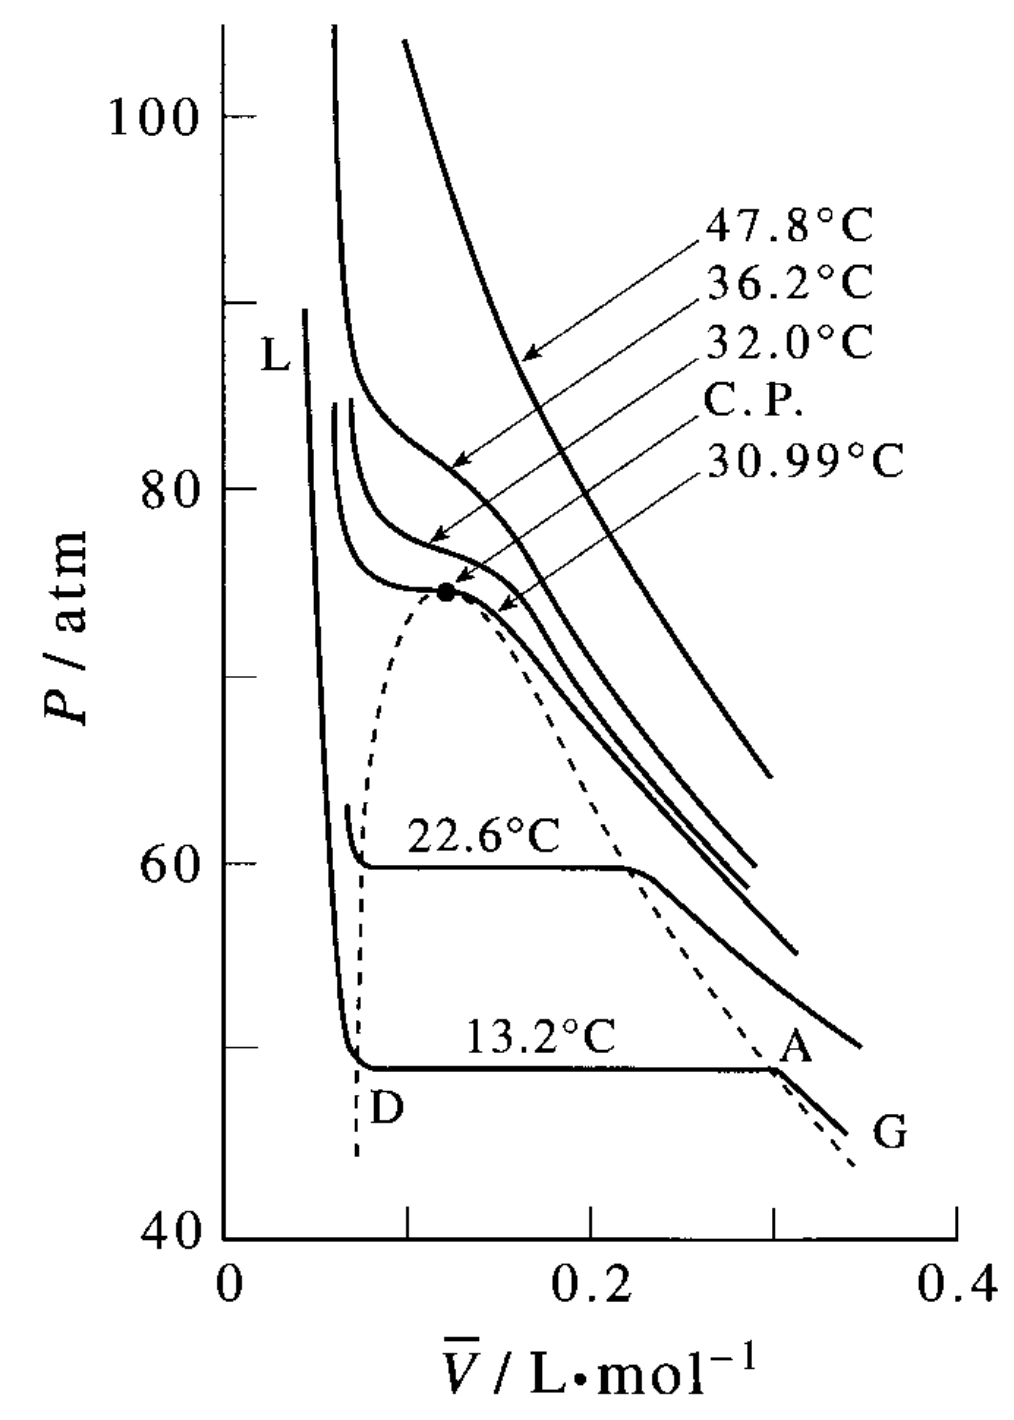
\includegraphics[width=0.28\linewidth]{../ExtFiles/PVterms.png}
        \caption{$PV$-diagram terminology.}
        \label{fig:PVterms}
    \end{figure}
    \item \textbf{Isotherm}: An experimentally determined plot of $P$ as a function of $\overline{V}$ at constant $T$.
    \item \textbf{Coexistence curve}: The curve on a $PV$ diagram such that any point within the curve corresponds to liquid and gas coexisting in equilibrium with each other and any point on or outside the curve corresponds to only one phase.
    \item \textbf{Critical temperature}: The temperature above which a gas cannot be liquefied, regardless of the pressure. \emph{Denoted by} $\bm{T_c}$.
    \item \textbf{Critical point}: The point along the curve $P(\overline{V},T_c)$ at which $\pdv*{P}{\overline{V}}=0$.
    \begin{itemize}
        \item The global maximum of the coexistence curve.
    \end{itemize}
    \item \textbf{Critical pressure}: The pressure at the critical point. \emph{Denoted by} $\bm{P_c}$.
    \item \textbf{Critical volume}: The volume at the critical point. \emph{Denoted by} $\bm{\overline{V}_c}$.
    \item \textbf{Critical density}: The density of the system at the critical point.
    \item \textcite{bib:McQuarrieSimon} describes how pressure remains constant during a phase transition at a subcritical temperature.
    \item At the critical point, the meniscus between liquid and vapor disappears and both take on the same critical density.
    \item The spurious loops obtained from the van der Waals and Redlich-Kwong equation for $T<T_c$ (see Figure \ref{fig:vanDerWaalsIsotherm}) result from the approximate nature of these equations of state.
    \begin{itemize}
        \item However, the segment AB is a metastable region corresponding to the superheated vapor, the segment CD corresponds to the supercooled liquid, and the segment BC signifies an unstable region not observed for equilibrium systems.
    \end{itemize}
    \item The \textbf{Maxwell equal-area construction} will be justified in Chapter 23.
    \item The three roots of the equations of state along isotherms for $T<T_c$.
    \begin{itemize}
        \item $A$ is the molar volume of the vapor in equilibrium.
        \item $D$ is the molar volume of the liquid in equilibrium.
        \item The third root in the middle has no physical meaning.
        \item We can thus use our cubic equations of state to calculate the molar volume of the liquid and gas phases of a given substance.
        \begin{itemize}
            \item Note that since it was designed to behave the best in the liquid region, the Peng-Robinson equation gives the best result here.
        \end{itemize}
    \end{itemize}
    \item Since the critical point is an inflection point along the isotherm corresponding to the critical temperature, we have that
    \begin{align*}
        \left( \pdv{P}{\overline{V}} \right)_T &= 0&
        \left( \pdv[2]{P}{\overline{V}} \right)_T &= 0
    \end{align*}
    at it.
    \begin{itemize}
        \item We can use these conditions to derive the critical constants in terms of $a$ and $b$.
    \end{itemize}
    \item An easier way to derive said expressions, though, is to note that the cubic van der Waals equation has three real roots for $T<T_c$ and one real root (plus two complex roots) for $T>T_c$, so at $T=T_c$, all three of its roots merge into one, i.e., the equation is of the form $(\overline{V}-\overline{V}_c)^3=0$.
    \begin{itemize}
        \item It follows by expanding the trinomial and comparing coefficients with the van der Waals equation written as a cubic that
        \begin{align*}
            3\overline{V}_c &= b+\frac{RT_c}{P_c}&
            3V_c^2 &= \frac{a}{P_c}&
            \overline{V}_c^3 &= \frac{ab}{P_c}
        \end{align*}
        \item It follows that
        \begin{align*}
            \overline{V}_c &= 3b&
            P_c &= \frac{a}{27b^2}&
            T_c &= \frac{8a}{27bR}
        \end{align*}
        \item For the Redlich-Kwong equation,
        \begin{align*}
            \overline{V}_c &= 3.8473B&
            P_c &= 0.029894\frac{A^{2/3}R^{1/3}}{B^{5/3}}&
            T_c &= 0.34504\left( \frac{A}{BR} \right)^{2/3}
        \end{align*}
    \end{itemize}
    \item From the above equations, we can show that
    \begin{align*}
        \frac{P_c\overline{V}_c}{RT_c} &= 0.375&
        \frac{P_c\overline{V}_c}{RT_c} &= 0.333
    \end{align*}
    where the left estimate is provided by the van der Waals equation and the right by the Redlich-Kwong equation.
    \begin{itemize}
        \item The significance is that both equations of state predict that the compressibility factor at the critical point is the same for all substances (there is no $a,b$ or $A,B$ dependence in the terms on the right of the equalities). However, there is a slight disparity in the predicted value of $Z$.
        \item While neither prediction is particularly quantitative (that of the Peng-Robinson is a bit more so), all three equations of state predict a constant $Z$. This prediction is borne out reasonably well by experimental data.
    \end{itemize}
    \item \textbf{Law of corresponding states}: The properties of all gases are the same if we compare them under the same conditions relative to their critical point.
    \begin{itemize}
        \item In particular, this means that gas properties are identical when their \textbf{reduced quantities} are equal.
    \end{itemize}
    \item Note that in practice, the van der Waals and Redlich-Kwong constants are obtained from data at the critical point, not the other way around.
    \begin{itemize}
        \item Also note that there is some ambiguity in how we do so, since there are three pieces of data $(P_c,\overline{V}_c,T_c)$ describing a gas at the critical point but only two constants $a,b$ or $A,B$.
    \end{itemize}
    \item \marginnote{2/25:}\textbf{Reduced quantity}: The quotient of a state variable of a gas and the value of that state variable for the gas at the critical point. \emph{Denoted by} $\bm{X_R}$ (if $X$ is a state variable).
    \begin{itemize}
        \item For example, the reduced pressure of a gas is $P_R=P/P_c$ where $P$ is its current pressure and $P_c$ is its critical pressure.
    \end{itemize}
    \item By recombining some of our previous equations, we can rewrite the van der Waals equation in the form
    \begin{equation*}
        \left( P_R+\frac{3}{\overline{V}_R^2} \right)\left( \overline{V}_R-\frac{1}{3} \right) = \frac{8}{3}T_R
    \end{equation*}
    \begin{itemize}
        \item Since the above equation doesn't contain any gas characteristics (e.g., $a,b,A,B,\alpha,\beta$), it is a universal equation for all gases.
        \item For example, it implies that any gas at the same reduced temperature and volume will have the same reduced pressure.
        \item This prediction is borne out by experimental data and forms the foundation of the law of corresponding states.
    \end{itemize}
    \item \textbf{Corresponding states} (of gases $A$ and $B$): A state $(P_A,V_A,T_A)$ of gas $A$ and $(P_B,V_B,T_B)$ of gas $B$ such that
    \begin{align*}
        P_{R_A} = \frac{P_A}{P_{c_A}} &= \frac{P_B}{P_{c_B}} = P_{R_B}&
        V_{R_A} = \frac{V_A}{V_{c_A}} &= \frac{V_B}{V_{c_B}} = V_{R_B}&
        T_{R_A} = \frac{T_A}{T_{c_A}} &= \frac{T_B}{T_{c_B}} = T_{R_B}
    \end{align*}
    \item The compressibility factor also obeys the law of corresponding states.
    \begin{figure}[h!]
        \centering
        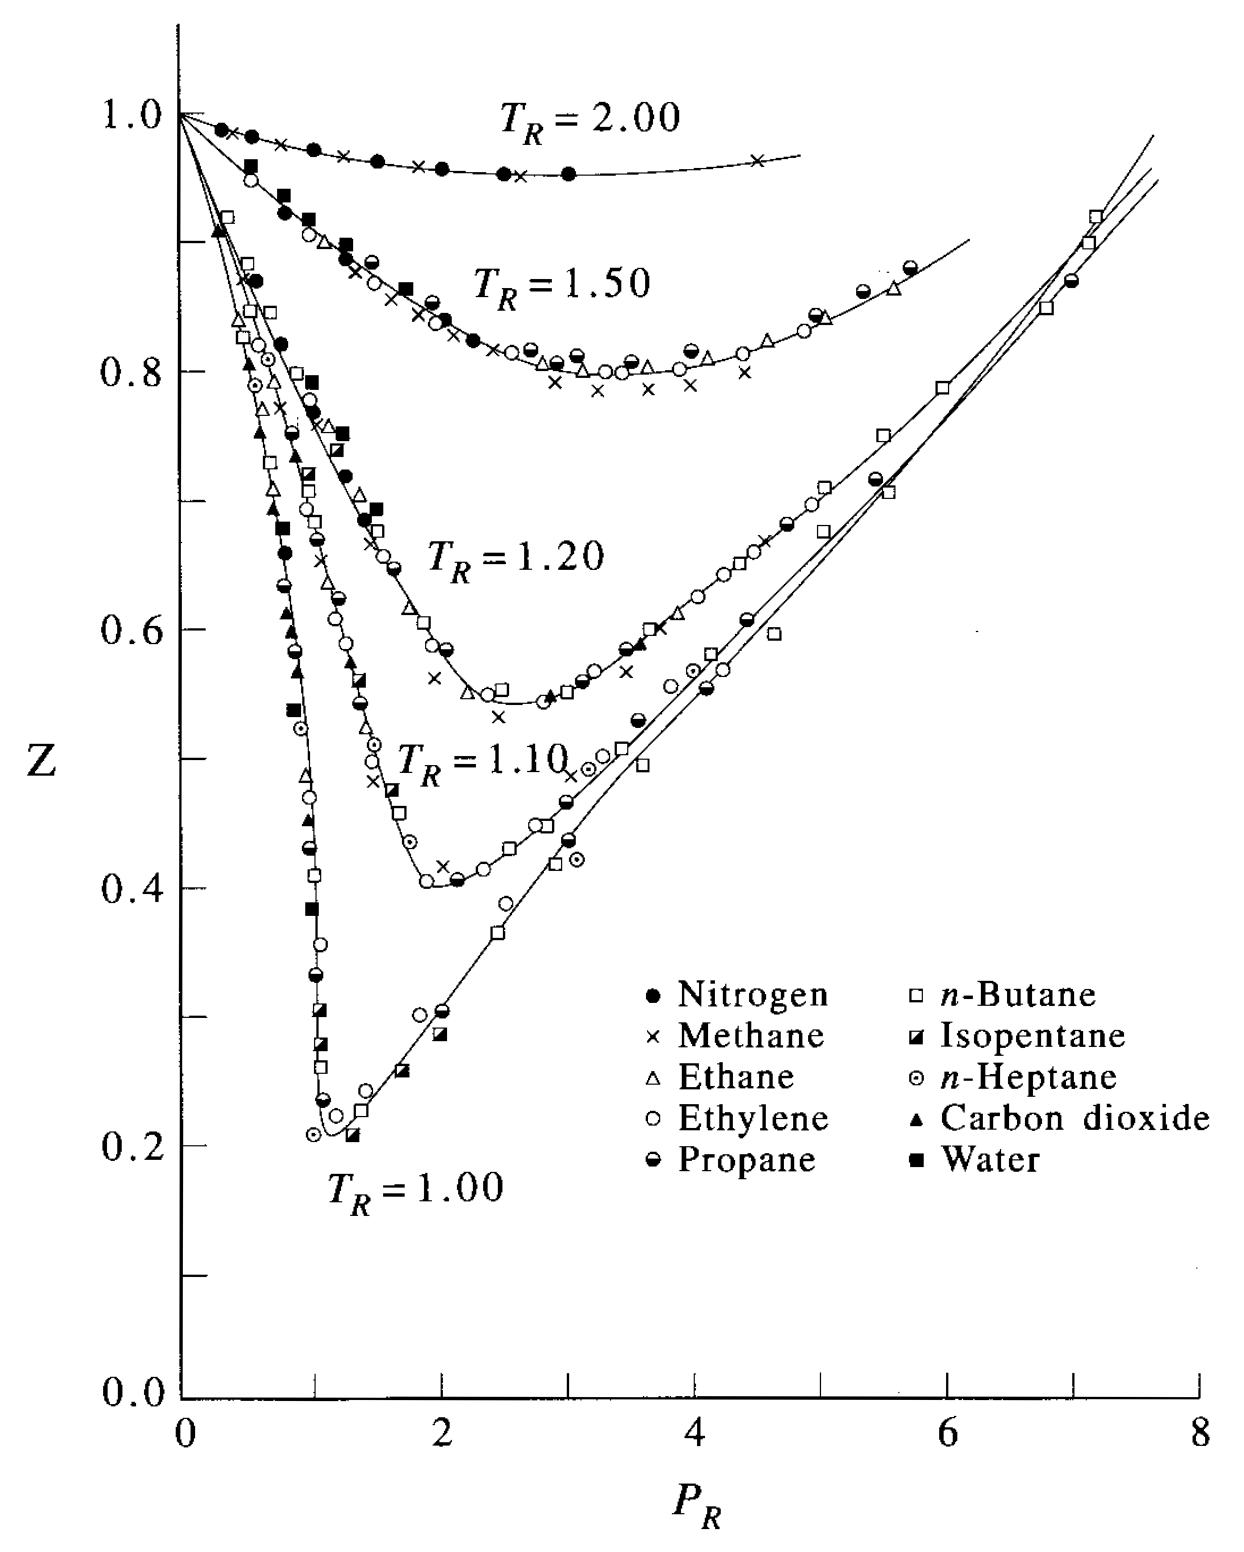
\includegraphics[width=0.5\linewidth]{../ExtFiles/lawCorrespondingStates.png}
        \caption{Experimental evidence for the law of corresponding states.}
        \label{fig:lawCorrespondingStates}
    \end{figure}
    \begin{itemize}
        \item For the van der Waals equation,
        \begin{align*}
            Z &= \frac{P\overline{V}}{RT}\\
            &= \frac{\overline{V}}{\overline{V}-b}-\frac{a}{RT\overline{V}}\\
            &= \frac{\overline{V}}{\overline{V}-\overline{V}_c/3}-\frac{3P_c\overline{V}_c^2}{RT\overline{V}}\\
            &= \frac{\overline{V}/\overline{V}_c}{\overline{V}/\overline{V}_c-1/3}-\frac{3\cdot 3RT_c/8\cdot\overline{V}_c}{RT\overline{V}}\\
            &= \frac{\overline{V}_R}{\overline{V}_R-1/3}-\frac{9}{8T_R\overline{V}_R}
        \end{align*}
        \item For the Redlich-Kwong equation,
        \begin{equation*}
            Z = \frac{\overline{V}_R}{\overline{V}_R-0.25992}-\frac{1.2824}{T_R^{3/2}(\overline{V}_R+0.25992)}
        \end{equation*}
    \end{itemize}
    \item Physical interpretation of the law of corresponding states: All temperature, pressure, volume, etc. scales on gases are arbitrary, even kelvin. The only values that matter as far as a gas is concerned are its reduced quantities.
    \item \textbf{Virial equation of state}: The most fundamental equation of state, i.e., the one with the most sound theoretical foundation. \emph{Given by}
    \begin{equation*}
        Z = \frac{P\overline{V}}{RT}
        = 1+\frac{B_{2V}(T)}{\overline{V}}+\frac{B_{3V}(T)}{\overline{V}^2}+\cdots
    \end{equation*}
    \item \textbf{Virial coefficients}: The coefficients in the above polynomial in $\overline{V}$.
    \item \textbf{$\bm{i^\textbf{th}}$ virial coefficient}: The virial coefficient $B_{iV}(T)$.
    \item \textbf{Virial expansion}: The expression of another property, such as energy or entropy, as a polynomial in $1/\overline{V}$.
    \item A useful virial expansion is the expression of $Z(P)$ given by
    \begin{equation*}
        Z = \frac{P\overline{V}}{RT}
        = 1+B_{2P}(T)P+B_{3P}(T)P^2+\cdots
    \end{equation*}
    where
    \begin{equation*}
        B_{iV}(T) = RTB_{iP}(T)
    \end{equation*}
    \item Note that in the above virial expansions, $\overline{V}\to\infty$ and $P\to 0$ as $Z\to 1$, as we would expect.
    \item The terms in the virial expansion converge rapidly.
    \item "The second virial coefficient is the most important virial coefficient because it reflects the first deviation from ideality as the pressure of the gas is increased (or the volume is decreased)" \parencite[659]{bib:McQuarrieSimon}.
    \begin{itemize}
        \item It can be measured from the slope of a plot of $Z$ vs. $P$ (at low pressures).
        \item $B_{2V}(T)$ is negative at low temperatures and increases with temperature, going through a shallow positive maximum and then decreasing asymptotically toward zero.
    \end{itemize}
    \item \textbf{Boyle temperature}: The temperature at which $B_{2V}(T)=0$, i.e., at which the repulsive and attractive parts of the intermolecular attractions cancel each other and the gas appears to behave ideally.
    \item The virial equation of state allows us to derive an exact relation between the virial coefficients and the intermolecular interactions.
    \begin{itemize}
        \item The interaction of two molecules depends on their distance apart and orientation in space. However, due to rapid molecular motion, we'll pretend that their orientation averages out (a good approximation for molecules of low polarity) and that only the intermolecular distance $r$ is important.
        \item Let $u(r)$ denote the potential energy of two molecules separated by a distance $r$. Then we can show that
        \begin{equation*}
            B_{2V}(T) = -2\pi\NA\int_0^\infty[\e[-u(r)/\kB T]-1]r^2\dd{r}
        \end{equation*}
        \item Note that as we'd expect, $B_{2V}(T)=0$ if $u(r)=0$, i.e., there are no deviations from ideality if there are no intermolecular interactions.
        \item In principle, $u(r)$ can be calculated from quantum mechanics, but this is complicated. Thus, we the approximation from perturbation theory that
        \begin{equation*}
            u(r) \to -\frac{c_6}{r^6}
        \end{equation*}
        for large values of $r$ where $c_6$ is a constant depending on the molecules in question.
        \begin{itemize}
            \item The negative sign represents attraction.
            \item At low temperatures, it is this attraction that leads to condensation.
        \end{itemize}
        \item Although there is no known exact expression for $u(r)$ at small distances, it must reflect intermolecular repulsions, so we usually choose
        \begin{equation*}
            u(r) \to \frac{c_n}{r^n}
        \end{equation*}
        for small $r$ where $n\in\N$ (but $n$ is often taken to be 12) and $c_n$, again, depends on the molecules in question.
        \item An intermolecular potential that accounts for both forces is the sum of the two, often written with the substitutions $c_{12}=4\varepsilon\sigma^{12}$ and $c_6=4\varepsilon\sigma^6$.
        \begin{equation*}
            u(r) = \frac{c_{12}}{r^{12}}-\frac{c_6}{r^6}
            = 4\varepsilon\left[ \left( \frac{\sigma}{r} \right)^{12}-\left( \frac{\sigma}{r} \right)^6 \right]
        \end{equation*}
    \end{itemize}
    \item \textbf{Lennard-Jones potential}: The above expression for $u(r)$ in terms of $\varepsilon$ and $\sigma$.
    \item \textbf{Lennard-Jones parameters}: The values $\varepsilon$ and $\sigma$.
    \begin{itemize}
        \item Let's calculate the value at which the Lennard-Jones potential achieves its minimum.
        \begin{align*}
            0 &= \dv{u}{r}\\
            &= 4\epsilon\left[ -\frac{12\sigma^{12}}{r^{13}}+\frac{6\sigma^6}{r^7} \right]\\
            \frac{12\sigma^{12}}{r^{13}} &= \frac{6\sigma^6}{r^7}\\
            2\sigma^6 &= r^6\\
            r_\text{min} &= 2^{1/6}\sigma
        \end{align*}
        \item It follows that
        \begin{equation*}
            u(r_\text{min}) = 4\epsilon\left[ \left( \frac{\sigma}{2^{1/6}\sigma} \right)^{12}-\left( \frac{\sigma}{2^{1/6}\sigma} \right)^6 \right]
            = 4\epsilon\left( \frac{1}{4}-\frac{1}{2} \right)
            = -\epsilon
        \end{equation*}
        i.e., that $\epsilon$ is the depth of the potential well relative to infinite separation.
        \begin{itemize}
            \item Thus, $\epsilon$ is a measure of how strongly the molecules attract each other.
        \end{itemize}
        \item Additionally, we have that
        \begin{equation*}
            u(\sigma) = 4\varepsilon\left[ \left( \frac{\sigma}{\sigma} \right)^{12}-\left( \frac{\sigma}{\sigma} \right)^6 \right] = 0
        \end{equation*}
        \begin{itemize}
            \item Thus, when $r=\sigma$, the intermolecular attraction and repulsion cancel, i.e., the molecules are finally close enough that their repulsion is becoming significant (in layman's terms, they're touching).
            \item This means that $\sigma$ is a measure of the size of the constituent molecules.
        \end{itemize}
    \end{itemize}
    \item Substituting the Lennard-Jones potential into our expression for $B_{2V}(T)$ in terms of $u(r)$ yields
    \begin{equation*}
        B_{2V}(T) = -2\pi\NA\int_0^\infty\left[ \exp\left\{ -\frac{4\varepsilon}{\kB T}\left[ \left( \frac{\sigma}{r} \right)^{12}-\left( \frac{\sigma}{r} \right)^6 \right] \right\}-1 \right]r^2\dd{r}
    \end{equation*}
    \item Substituting a reduced temperature $T^*=\kB T/\varepsilon$, $x=r/\sigma$, and a reduced second virial coefficient $B_{2V}^*(T^*)=B_{2V}(T^*)/(2\pi\sigma^3\NA/3)$ yields
    \begin{equation*}
        B_{2V}^*(T^*) = -3\int_0^\infty\left[ \exp\left\{ -\frac{4}{T^*}(x^{-12}-x^{-6}) \right\}-1 \right]x^2\dd{x}
    \end{equation*}
    where the integral must be evaluated numerically for each $T^*$. Extensive tabulations of these values are available, though.
    \begin{itemize}
        \item Note that this equation is another example of the law of corresponding states. Plotting $B_{2V}^*(T^*)$ vs. $T^*$ for almost any gas will generate much the same curve.
    \end{itemize}
    \item Another interpretation of $B_{2V}(T)$.
    \begin{itemize}
        \item Consider the virial expansion in terms of pressure under conditions such that terms $P^2$ and higher are negligible. Then
        \begin{align*}
            \frac{P\overline{V}}{RT} &= 1+B_{2P}(T)P\\
            &= 1+\frac{B_{2V}(T)}{RT}P\\
            \overline{V} &= \frac{RT}{P}+B_{2V}(T)\\
            B_{2V}(T) &= \overline{V}-\overline{V}_\text{ideal}
        \end{align*}
    \end{itemize}
    \item Note that in much the same way we actually use critical point information to calculate van der Waals and Redlich-Kwong constants, we actually use $B_{2V}(T)$ data to calculate Lennard-Jones parameters.
    \item "Because the second virial coefficient reflects the initial deviations from ideal behavior, which are caused by intermolecular interactions, experimental $P$-$V$-$T$ data turn out to be a rich source of information concerning intermolecular interactions" \parencite[665]{bib:McQuarrieSimon}.
    \begin{itemize}
        \item Once the Lennard-Jones parameters of a substance are known, they can be used to calculate properties such as viscosity, thermal conductivity, heats of vaporization, and various crystal properties.
    \end{itemize}
    \item We now consider in more depth the form of the $r^{-6}$ attraction term.
    \item Consider two molecules with dipoles $\mu_1,\mu_2$.
    \begin{itemize}
        \item If we assume that these molecules rotate randomly in the gas phase, their average dipole-dipole interactions would be zero.
        \item However, because different conformations (e.g. head-to-head vs. head-to-tail) have different energies, the various states do not occur with equal probabilities. This gives us the following expression for the average interaction between two molecular dipoles.
        \begin{equation*}
            u_{d.d}(r) = -\frac{2\mu_1^2\mu_2^2}{(4\pi\varepsilon_0)^2(3\kB T)}\frac{1}{r^6}
        \end{equation*}
    \end{itemize}
    \item Consider two molecules, one with a permanent dipole and the other without a permanent dipole.
    \begin{itemize}
        \item Dipole moments can be induced in molecules without a permanent one since all atoms and molecules are \textbf{polarizable}.
        \item Thus,
        \begin{equation*}
            u_\text{induced}(r) = -\frac{\mu_1^2\alpha_2}{(4\pi\varepsilon_0)^2r^6}-\frac{\mu_2^2\alpha_1}{(4\pi\varepsilon_0)^2r^6}
        \end{equation*}
        \item The first term above represents a permanent dipole moment in molecule 1 and an induced dipole moment in molecule 2, and the second represents the opposite situation.
    \end{itemize}
    \item \textbf{Polarizability}: The proportionality constant between the induced dipole moment $\mu_\text{induced}$ and the external electric field strength $E$. \emph{Denoted by} $\bm{\alpha}$.
    \begin{itemize}
        \item "The easier it is for the electric field to deform the atomic or molecular charge distribution, the greater is the polarizability" \parencite[667-68]{bib:McQuarrieSimon}.
    \end{itemize}
    \item \textbf{Polarizability volume}: The quantity $\alpha/4\pi\varepsilon_0$, which has units of volume.
    \begin{itemize}
        \item The polarizability of an atom or molecule is proportional to its size, hence another reason for introducing the polarizability volume.
    \end{itemize}
    \item Consider two molecules, neither of which has a permanent dipole.
    \begin{itemize}
        \item Because of the \textbf{London dispersion attraction}, their energy of interaction is
        \begin{equation*}
            u_\text{disp}(r) = -\frac{3}{2}\left( \frac{I_1I_2}{I_1+I_2} \right)\frac{\alpha_1\alpha_2}{(4\pi\varepsilon_0)^2}\frac{1}{r^6}
        \end{equation*}
        where $I_j$ is the ionization energy of atom or molecule $j$.
        \item Since $u_\text{disp}$ is proportional to the product of the polarizability volumes, the importance of $u_\text{disp}$ increases with the sizes of the atoms or molecules.
    \end{itemize}
    \item \textbf{London dispersion attraction}: A strictly quantum-mechanical effect that draws all molecules together, even nonpolar ones.
    \begin{itemize}
        \item Named for the German scientist Fritz London who first calculated it in 1930.
        \item Note that the classical picture taught in intro chem of electrons and protons shifting isn't strictly accurate --- it's more about the distortion/perturbation of wave functions as particles draw near.
    \end{itemize}
    \item It follows that the total contribution to the $r^{-6}$ term of the Lennard-Jones potential is given by the sum of the previous three results, i.e.,
    \begin{equation*}
        c_6 = \frac{2\mu^4}{3(4\pi\varepsilon_0)^2\kB T}+\frac{2\alpha\mu^2}{(4\pi\varepsilon_0)^2}+\frac{3}{4}\frac{I\alpha^2}{(4\pi\varepsilon_0)^2}
    \end{equation*}
    for identical atoms and molecules.
\end{itemize}




\end{document}